\section{MOS Stromspiegel\skript{Kap. 9}}
Ziel: Aus einer einzelnen genauen Strom- oder Spannungsquelle verschiedene genaue Ströme erzeugen.

\begin{tabularx}{\linewidth}{|l|l|X|}
	\hline
	Stromspiegelverhältnis & $n_m$ & $n_m = \frac{I_0}{I_i} = \frac{(\frac{W}{L})_{out}}{(\frac{W}{L})_{in}} \approx \frac{i_0}{i_i}$
	\\ \hline
\end{tabularx}

\subsection{Die wichtigsten Formeln}
\begin{multicols}{2}
	\textbf{Stromspiegelverhältnis}
	\[
		n_m = \frac{I_o}{I_i} 
			= \frac{\left(\frac{W}{L}\right)_o}{\left(\frac{W}{L}\right)_i}
			= \frac{I_{Do}}{I_{Di}}
	\]
	\\
		
	\textbf{Berechnung Ausgangsstrom}
	\[
		I_{out} = I_{in}\cdot\frac{W_{T_{out}}}{W_{T_{in}}}
	\]
	gilt nur wenn $L_{T_{out}} = L_{T_{in}}$ \\

	\columnbreak
	\textbf{ESB des Widlar-Stromspiegels} \\
		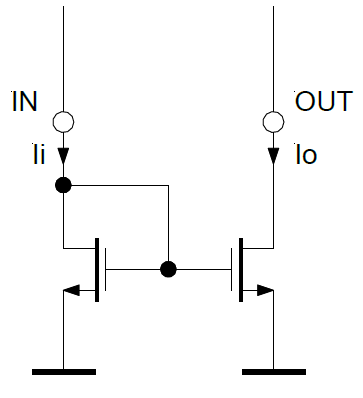
\includegraphics[width=3cm]{images/stromspiegel/widlar_n.png} \\
		\adjustbox{scale=0.7}{\begin{circuitikz}[american, european resistors]
	\draw (0,0) node[circ] {} node[right] {IN};
	\draw (0,0) -- (0,-0.5);
	\draw (0,-0.5) to[R=$1/g_m$,i>^=$I_B$] (0,-2.5);
	\draw (2,0) node[circ] {} node[right] {OUT};
	\draw (2,0) -- (2,-0.5);
	\draw (2,-0.5) to[I,l=$n_m I_B$] (2,-2.5);
	\draw (0,-2.5) -- (2,-2.5);
\end{circuitikz}}
\end{multicols}


\begin{tabular}{|l|c|l|l|l|}
	\hline
	\textbf{Stromspiegeltyp} & \textbf{Genauigkeit} & \boldmath{$r_{out}$} & \boldmath{$V_I$} & \boldmath{$V_{O,min}$}
	\\ \hline
	Widlar Stromspiegel		& $+$	& $= \frac{1}{g_0}$								& $\approx V_T + \sqrt{\frac{2I_I}{\beta}}$		& $\approx \sqrt{\frac{2I_0}{\beta}}$
	\\ \hline
	Wilson Stromspiegel		& $+$	& $\approx \frac{1}{g_0}(2 + \frac{g_m}{g_0})$	& $\approx 2V_T + 2\sqrt{\frac{2I_I}{\beta}}$	& $\approx V_T + 2\sqrt{\frac{2I_0}{\beta}}$
	\\ \hline
	Verbesserter Wilson		& $++$	& $\approx \frac{1}{g_0}(2 + \frac{g_m}{g_0})$	& $\approx 2V_T + 2\sqrt{\frac{2I_I}{\beta}}$	& $\approx V_T + 2\sqrt{\frac{2I_0}{\beta}}$
	\\ \hline
	Kaskode-Stromspiegel	& $++$	& $\approx \frac{1}{g_0}(2 + \frac{g_m}{g_0})$	& $\approx 2V_T + 2\sqrt{\frac{2I_I}{\beta}}$	& $\approx V_T + 2\sqrt{\frac{2I_0}{\beta}}$
	\\ \hline
	geregelte Kaskode		& $++$	& $\approx \frac{1}{g_0}(\frac{g_m}{g_0})^2$	& $\approx V_T + \sqrt{\frac{2I_I}{\beta}}$		& $\approx 2\sqrt{\frac{2I_0}{\beta}}$
	\\ \hline
\end{tabular}

\begin{figure}[h]
	\centering
	\begin{subfigure}[b]{5cm}
		\centering
		{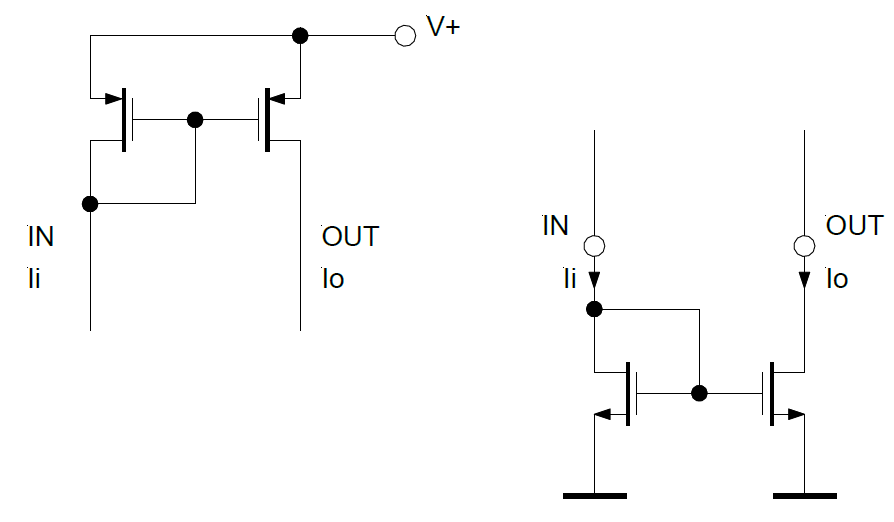
\includegraphics[width=5cm]{images/stromspiegel/widlar.png}}
		\caption{Widlar}
	\end{subfigure} \qquad	
	\begin{subfigure}[b]{5cm}
		\centering
		{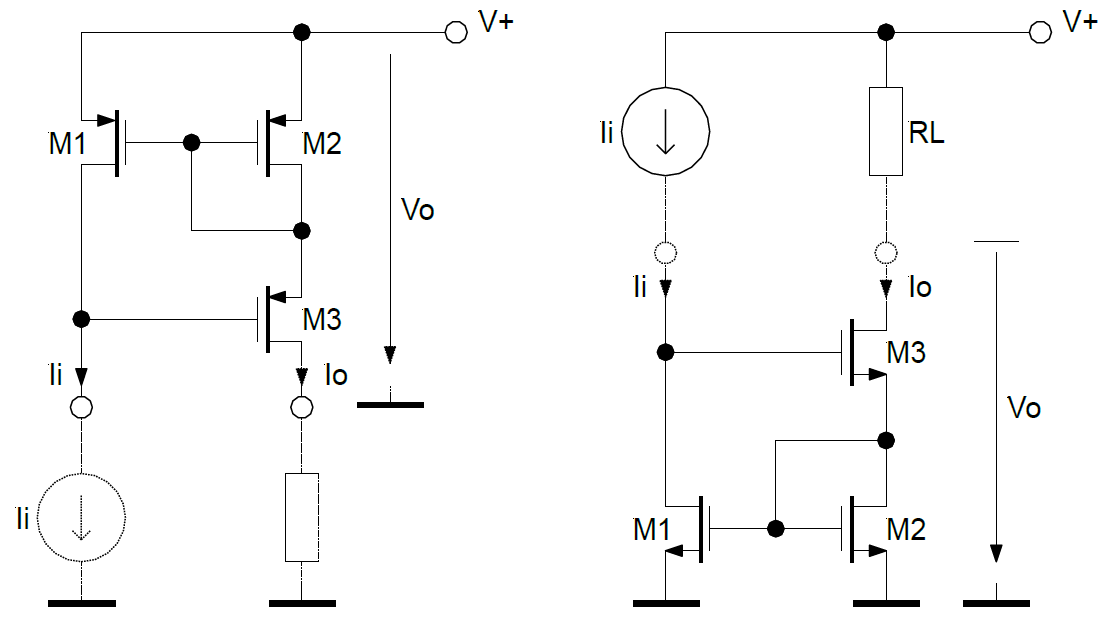
\includegraphics[width=5cm]{images/stromspiegel/wilson.png}}
		\caption{Wilson}
	\end{subfigure}
	
	\begin{subfigure}[b]{5cm}
		\centering
		{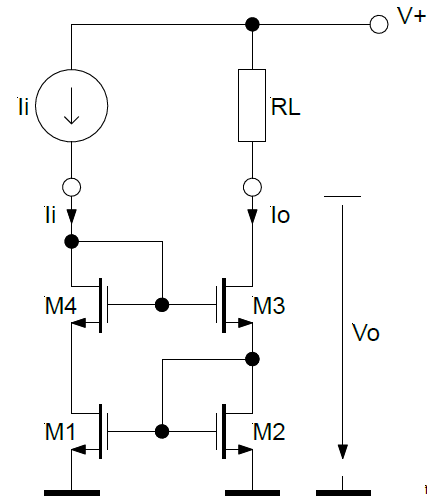
\includegraphics[width=3cm]{images/stromspiegel/verbesserter_wilson.png}}
		\caption{Verbesserter Wilson}
	\end{subfigure} \qquad	
	\begin{subfigure}[b]{3cm}
		\centering
		{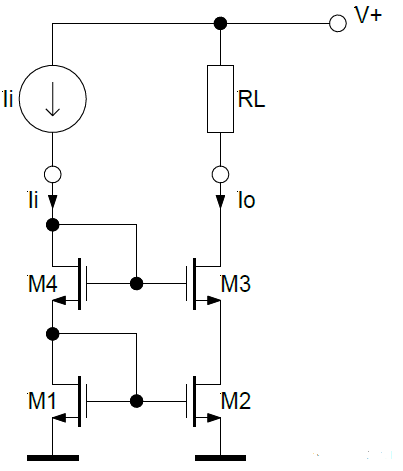
\includegraphics[width=3cm]{images/stromspiegel/kaskode.png}}
		\caption{Kaskode}
	\end{subfigure} \qquad	
	\begin{subfigure}[b]{3cm}
		\centering
		{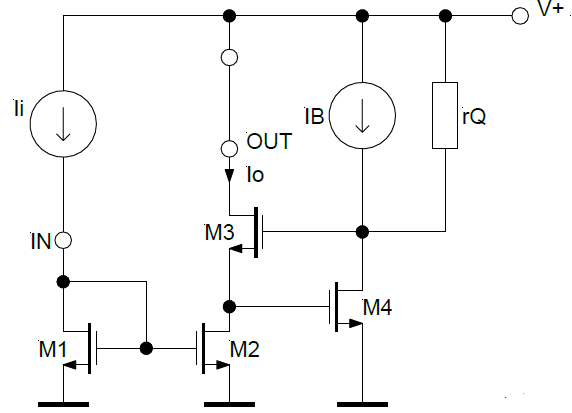
\includegraphics[width=3cm]{images/stromspiegel/geregelte_kaskode.png}}
		\caption{Geregelte Kaskode}
	\end{subfigure} 

	\caption{Die Stromspiegeltypen}
	\label{fig:stromspiegeltypen}
\end{figure}